\chapter{Experiment and Evaluation - User Study}
In this chapter, the Graphy prototype is evaluated in a user study. The objective of the study is to evaluate the user acceptance of Graphy to see whether it achieves its three goals: allowing users to find contacts by their miscellaneous information, efficiently retain knowledge of contacts, and enabling users to establish relationships between contacts then traverse the relationships with ease. The chapter contains three sections describing the hypotheses of the study, the detailed experimental setup, and the results.
\section{Hypotheses}
The main goal of this user study is to evaluate Graphy's functionalities in real use over a period of time. The evaluation mainly aims at testing the following hypotheses:
\begin{enumerate}
  \item Graphy allows users to find contacts by their miscellaneous information. Users often use this functionality.
  \item Graphy allows users to efficiently retain knowledge of contacts. Users utilize this feature to maintain a considerable amount of information, especially miscellaneous information.
  \item Graphy allows users to establish relationships between contacts then traverse the relationship network with ease. Users create a lot of relationships and actively traverse the relationships during their usage.
\end{enumerate}
\section{Experimental Setup}
The method of this user study is to recruit people to download the Graphy application to their smart phones after signing a consent form to participate in the study. The participants then use it in an uncontrolled environment for two weeks. The Graphy application records users' activities like creating, editing, and searching for contacts into a list of numbers on a summary screen which is part of the user interface. After using it for two weeks, the users go to the summary screen and copy all the numbers on it to an online form. The summary screen and the online form are illustrated in figures \ref{fig:summary_page}) and \ref{fig:survey_form}).

\begin{figure}[!h]
\begin{centering}
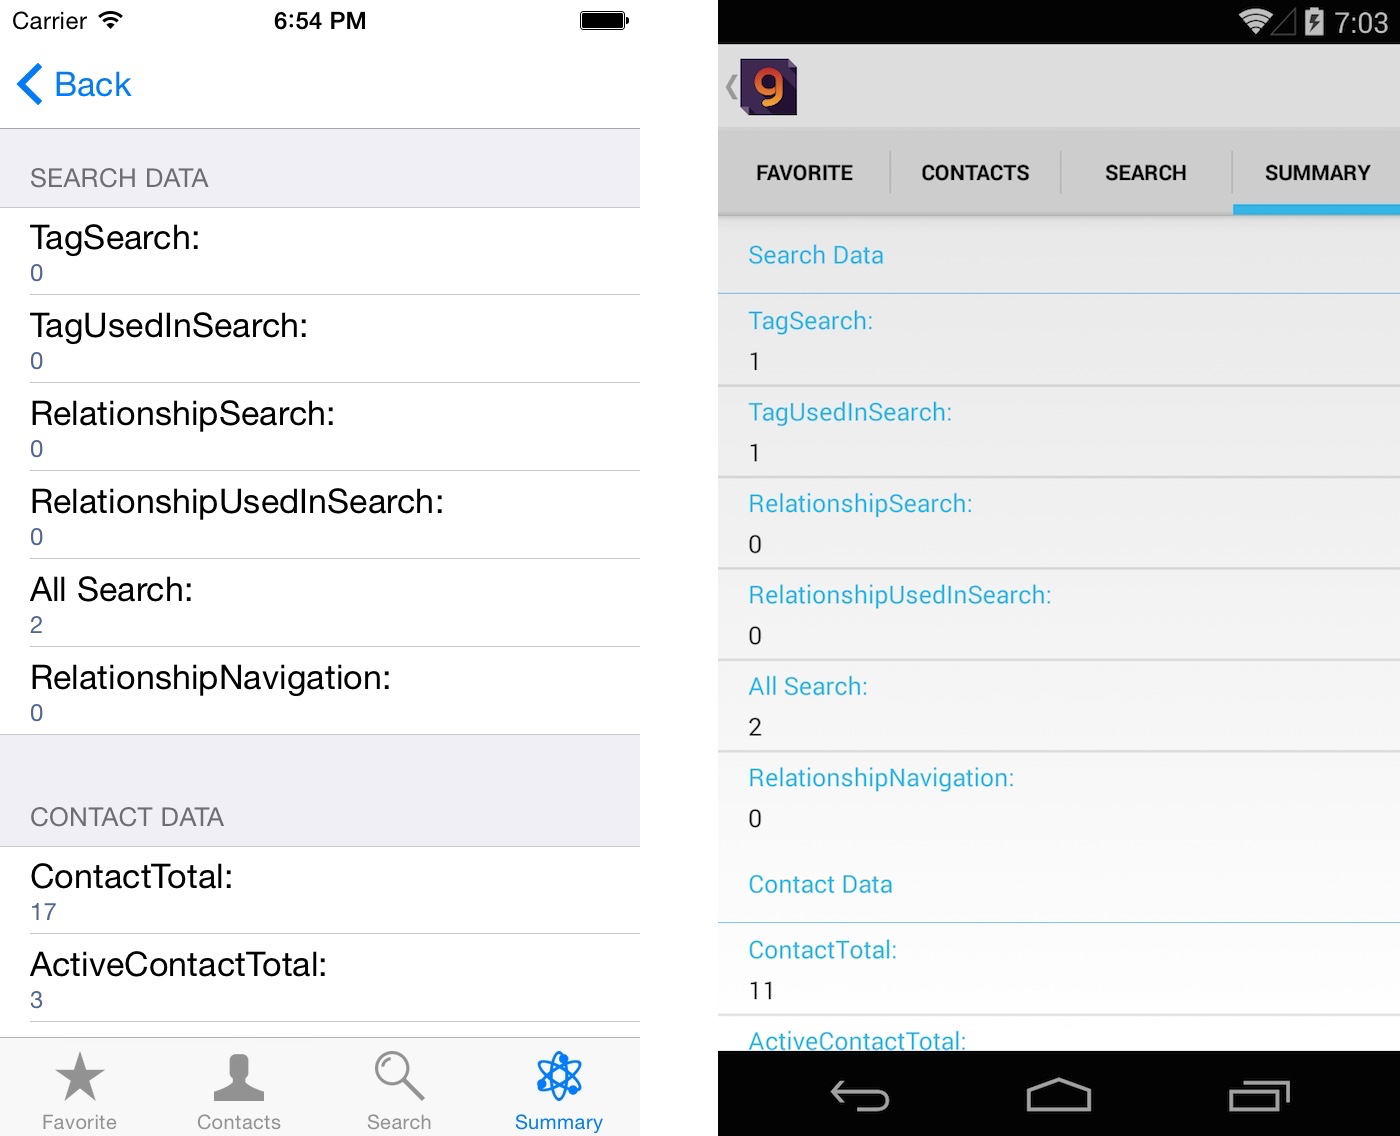
\includegraphics[scale=0.33]{pics/summary_page.png}
\caption{Graphy's Summary Page}\label{fig:summary_page}
\end{centering}
\end{figure}

\begin{figure}[!h]
\begin{centering}
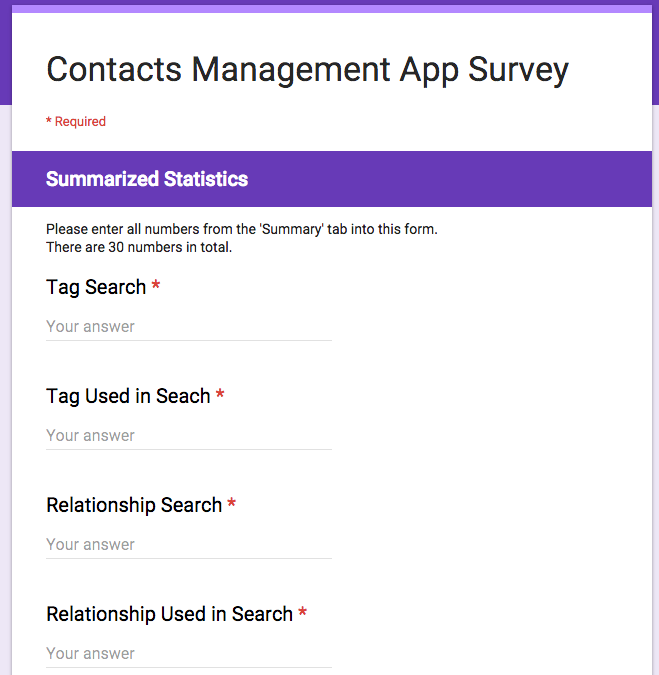
\includegraphics[scale=0.6]{pics/survey_form.png}
\caption{Graphy's Online Form}\label{fig:survey_form}
\end{centering}
\end{figure}

To recruit participants, we sent email invitations to our contacts list and also advertised the study on Facebook. As a result, twenty one people installed the application and finished the online form. The form is divided into two categories: one for tags (which represent pieces of miscellaneous information), one for relationships. Each category has two sections: the contact data and the search pattern. The contact data section accumulates information in the users' contacts list. For example, it records the total number of contacts, the total number of tags and relationships created during the study. This section allows us to examine the way participants store their information using Graphy, how they utilize the newly introduced elements in our application. The search pattern section collects data when a participant uses the search function or traverse the relationships network. For example, it tracks the frequency a user searches for contacts using tags, the number of tags used in each search, and how many times the user navigates from one contact to another through the relationship network. This section helps us to understand how people consume the data they store in Graphy: whether they use the newly introduced elements to search or they still use traditional information like first name and last name, whether they use the relationships network to look for a contact, etc.
\section{Results and Discussion}
This section presents the results of the study. The section contains four parts. The first part \textit{Tags and Relationships} \ref{results_tags_relationships} looks into the information participants store in Graphy which includes tags, relationships, and traditional information like names and phone numbers. The second part \textit{Search Pattern} \ref{results_search} examines how participants consume the data they stored in Graphy through searching and navigating the relationships network. The third part \textit{General Feedbacks and Discussion} \ref{results_feedbacks} analyzes some general feedbacks we received from the users then discusses the strengths and weaknesses of the study. The last part summarizes what we achieve through this user study.
\subsection{Tags and Relationships}\label{results_tags_relationships}
The first few metrics of Graphy aim to evaluate how intensively the participants use the system. More specifically, the first metric that we calculate is Active Contacts Total - the total number of contacts which were viewed, edited or added during the study. All data from the twenty one respondents shows a moderately high number of Active Contacts Total. On average, a person use approximately 33 contacts in 2 weeks, which is well over 2 contacts per day. The vast majority of the users have more than 15 active contacts as opposed to only a modest 14\% of them have less than 15. The Active Contacts Total data can be seen in Table \ref{table:active_contacts} and the group of Figures \ref{fig:active_contacts}, \ref{fig:tags_total}, \ref{fig:relationships_total}. From the data, we can infer that participants use Graphy quite a lot. 

\begin{table}[htbp]
  \centering
  \caption{Total Numbers of Active Contacts, Tags, and Relationships}\label{table:active_contacts} 
    \begin{tabular}{rrrrr}
    \toprule
    Active Contacts Total & Tags Total & Tags Average & Relationships Total & Relationships Average \\
    \midrule
    46    & 180   & 3.913 & 94    & 2.0435 \\
    72    & 241   & 3.3472 & 146   & 2.0278 \\
    55    & 127   & 2.3091 & 67    & 1.2182 \\
    16    & 27    & 1.6875 & 30    & 1.875 \\
    50    & 101   & 2.02  & 87    & 1.74 \\
    9     & 22    & 2.4444 & 7     & 0.7778 \\
    8     & 29    & 3.625 & 12    & 1.5 \\
    49    & 165   & 3.3673 & 86    & 1.7551 \\
    20    & 48    & 2.4   & 39    & 1.95 \\
    18    & 69    & 3.8333 & 34    & 1.8889 \\
    32    & 68    & 2.125 & 45    & 1.4063 \\
    29    & 67    & 2.3103 & 33    & 1.1379 \\
    23    & 60    & 2.6087 & 29    & 1.2609 \\
    24    & 47    & 1.9583 & 38    & 1.5833 \\
    30    & 102   & 3.4   & 58    & 1.9333 \\
    63    & 207   & 3.2857 & 128   & 2.0317 \\
    8     & 26    & 3.25  & 10    & 1.25 \\
    52    & 111   & 2.1346 & 80    & 1.5385 \\
    41    & 85    & 2.0732 & 71    & 1.7317 \\
    22    & 41    & 1.8636 & 41    & 1.8636 \\
    17    & 56    & 3.2941 & 31    & 1.8235 \\
          &       &       &       &  \\
    \textbf{32.5714} &  \textbf{89.4762} &  \textbf{2.7262} &  \textbf{55.5238} &  \textbf{1.6351} \\
    \bottomrule
    \end{tabular}%
  \label{tab:addlabel}%
\end{table}%

Table \ref{table:active_contacts} also shows the other two metrics: Tags Total and Relationships Total which are the total number of tags and relationships respectively. Regarding tags, the average total number is almost 90. A significant proportion of participants, 38\%, maintain more than 100 tags. Nobody has less than 20 tags and 2 people strikingly have more than 200 tags. Diviving the number of tags to the number of active contacts gives us the average of tags per contact which we call Tag Average. To be more specific, the Tag Average among all participants is roughly 2.73 tags per contact. The highest Tag Average is 3.91 and the lowest is 1.68. These are promising numbers. Generally, every user creates at least one tag for his/her contacts and on average almost 3 tags per contact. Because tags represent miscellaneous information users put into their contacts, the higher the numbers, the more miscellaneous information is created. From the collected data here, we can conclude that participants need about 3 pieces of miscellaneous information for every contact. Notably, the tags recorded here are not including Auto Added Tag (tags that the system automatically adds to a contact like \textit{Date Created}, \textit{Location Created}). In comparison with tags, the numbers of relationships are slightly smaller. On average, a respondent creates 55.52 relationships over the course of 14 days. Only 2 users, that is 9.5\%, maintain more than 100 relationships. When it comes to Relationship Average, typically each contact has 1.63 relationships. There are three people maintaining the highest Relationship Averages at 2.02, 2.03, and 2.04. On the contrary, there is one person has only 0.78 relationships per contact. Although the users tends to create fewer relationships than tags, 1.63 relationship per contact is still a very positive indicator.

\begin{figure}[!htbp]
\begin{centering}
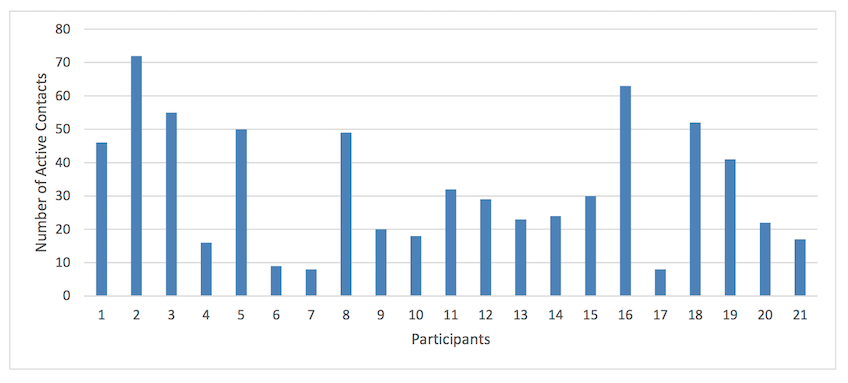
\includegraphics[scale=0.5]{pics/active_contacts.png}
\caption{Number of Active Contacts}\label{fig:active_contacts}
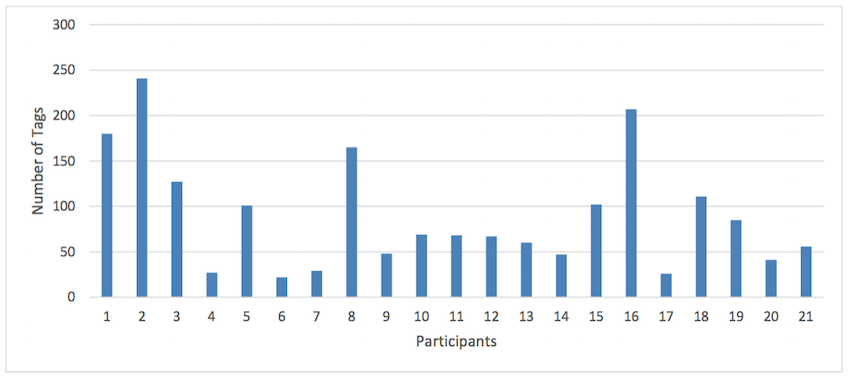
\includegraphics[scale=0.5]{pics/tags_total.png}
\caption{Number of Tags}\label{fig:tags_total}
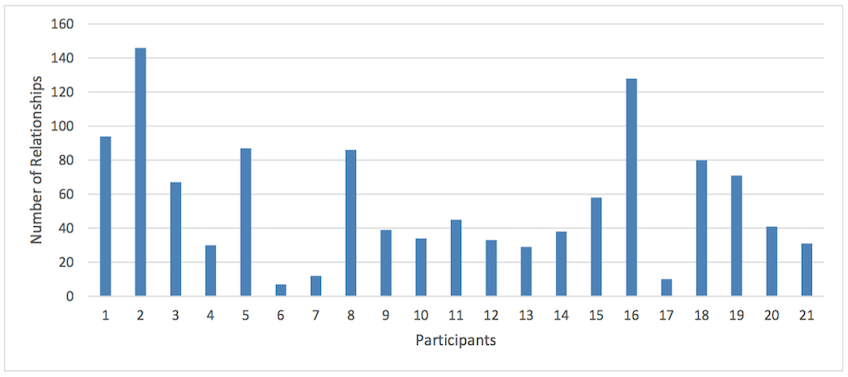
\includegraphics[scale=0.5]{pics/relationships_total.png}
\caption{Number of Relationships}\label{fig:relationships_total}
\end{centering}
\end{figure}

Beside calculating the total numbers of tags and relationships, we also record tag and relationship types. Table \ref{table:tag_relationship_types} shows how many types of tags and relationships were created during the experiment. The Average Tag Type Count is about 65. The person with the most tag types has 126 types while the person creates the least types has 27. Another thing which stands out in this table is that there are two people who have more tag types than tags. They both have very small numbers of tag types which are 29 and 30. These unusual situations can be explained by two reasons. First, Graphy has 4 pre-defined tags which are hard-coded in the application: \textit{Colleague}, \textit{Important}, \textit{Created Date}, \textit{Created Location}. We create these pre-defined tags as examples to guide users on how to use tags. These 4 tags are added to the number of tag types so it is possible that the users get 4 extra types without actually using them. Second, every time a user creates a tag type, the type is stored in the database so the user can use it for multiple contacts. If the user creates some types then never uses them, or uses the types on a contact then deletes that contact, the total number of tag types will be increased by the amount of unused types. This fact reveals a limitation in our system design. Ideally, Graphy should have a clean up function which deletes unused types after a long period of time. To some extent, the ratio of the number of tags to the number of tag types implies how many times a tag is reused. From table \ref{table:tag_relationship_types}, the average ratio is roughly 1.3 tag for each tag type. Noticeably, there is one participant maintains a ratio of exactly 1. Overall, this ``reuse'' ratio is fairly low. On the one hand, that means miscellaneous information is broad and needs many different tag types to cover. On the other hand, it exposes another limitation of the system: poor recommendation for tag/relationship types. At the moment, our application lets people enter new tag type names or pick an existing tag type from a list. A better solution should be suggesting existing types as users entering type names. Moreover, Graphy is currently case sensitive which in turn may be inflexible. For instance, it will consider these two names different types ``Important'' and ``important''. Therefore, making Graphy case-insensitive or equipping it with the capability of detecting similar words is quite important. These two improvements will be reserve for future work. In comparison to tag type, the number of relationship types is smaller by a large margin. The average number of relationship types is only 17, nearly 4 times smaller than the tag types. Turning to the relationships reuse ratio, it is just almost three times as big as the ratio of tags. Notably, there is one respondent having the the relationship reuse ratio of 7.9 which is substantially high. Furthermore, the lowest relationship reuse ratio is practically 2 relationships for each relationship type. These numbers suggest that relationship types are very well used, and people appear to have less kinds of relationship.

\begin{table}[!htbp]
  \centering
  \caption{Tag and Relationship Types}\label{table:tag_relationship_types} 
    \begin{tabular}{rrrrrr}
    \toprule
    Tag Total & \specialcell[t]{Tag:\\Type Count} & \specialcell[t]{Tag:\\Total/Type} & Relationship Total & \specialcell[t]{Relationship:\\Type Count} & \specialcell[t]{Relationship:\\Total/Type} \\
    \midrule
    180   & 114   & 1.5789 & 94    & 23    & 4.087 \\
    241   & 106   & 2.2736 & 146   & 36    & 4.0556 \\
    127   & 126   & 1.0079 & 67    & 36    & 1.8611 \\
    27    & 27    & 1     & 30    & 14    & 2.1429 \\
    101   & 91    & 1.1099 & 87    & 11    & 7.9091 \\
    22    & 29    & 0.7586 & 7     & 4     & 1.75 \\
    29    & 30    & 0.9667 & 12    & 5     & 2.4 \\
    165   & 117   & 1.4103 & 86    & 27    & 3.1852 \\
    48    & 39    & 1.2308 & 39    & 15    & 2.6 \\
    69    & 52    & 1.3269 & 34    & 10    & 3.4 \\
    68    & 67    & 1.0149 & 45    & 23    & 1.9565 \\
    67    & 64    & 1.0469 & 33    & 18    & 1.8333 \\
    60    & 42    & 1.4286 & 29    & 15    & 1.9333 \\
    47    & 39    & 1.2051 & 38    & 17    & 2.2353 \\
    102   & 56    & 1.8214 & 58    & 16    & 3.625 \\
    207   & 94    & 2.2021 & 128   & 33    & 3.8788 \\
    26    & 20    & 1.3   & 10    & 5     & 2 \\
    111   & 104   & 1.0673 & 80    & 20    & 4 \\
    85    & 78    & 1.0897 & 71    & 10    & 7.1 \\
    41    & 39    & 1.0513 & 41    & 13    & 3.1538 \\
    56    & 45    & 1.2444 & 31    & 10    & 3.1 \\
          &       &       &       &       &  \\
    \textbf{89.4762} & \textbf{65.6667} & \textbf{1.2922} & \textbf{55.5238} & \textbf{17.1905} & \textbf{3.2479} \\
    \bottomrule
    \end{tabular}%
  \label{tab:addlabel}%
\end{table}%

When it comes to measuring the impact of Graphy's new elements to a contact, we use another two metrics: Tag Weight Average and Relationship Weight Average. The way these metrics are calculated is as follows: on a contact we count the number of tag fields and the number of relationship fields then divide them to the number of all fields from which we get Tag Weight and Relationship Weight. The averages of Tag and Relationship Weight are then computed among all the contacts of a participant. The histograms of the two metrics are illustrated with Figure \ref{fig:tag_weight_histogram} and \ref{fig:relationship_weight_histogram} while the detailed results can be found in Appendix A. As regards Tag Weight Average, each participant generally maintain a considerable high number at roughly 27\%. Remarkably, the vast majority of participants (10 people) have Tag Weight Average between 31\% and 35\%. Nobody has less than 16\% or more than 40\% on this metric. It is worth noting that Auto Added Tags such as \textit{Date Created} and \textit{Location Created} are not included in the calculation. If we add these two simple tags into the formula, Tag Weight Average can be increased by a large margin. By comparison, Relationship Weight is a little lower than Tag Weight at approximately 17\%. Only one respondent has Relationship Weight Average less than 10\% while the greatest proportion of respondents, 57\% (12 people), keep this metric in the 16-20\% range. There are four users with Tag Weight Average between 11\% and 15\%, at the same time another four users have the metric between 21\% and 25\%. The data is again very promising. On average, tags and relationships together serve almost half the information in a contact. The pie chart \ref{fig:average_contact_fields} displays more clearly that Graphy's newly introduced elements (tags and relationships) are practically as many as traditional pieces of information (e.g. names, phone numbers, emails, etc.). From our experience, a contact typically contains 3 to 5 traditional fields: a first name and last name, one or two phone numbers, an email, and sometimes the organization that contact belongs to (interestingly, the organization is often placed together with the name). 

\begin{figure}[!h]
\begin{centering}
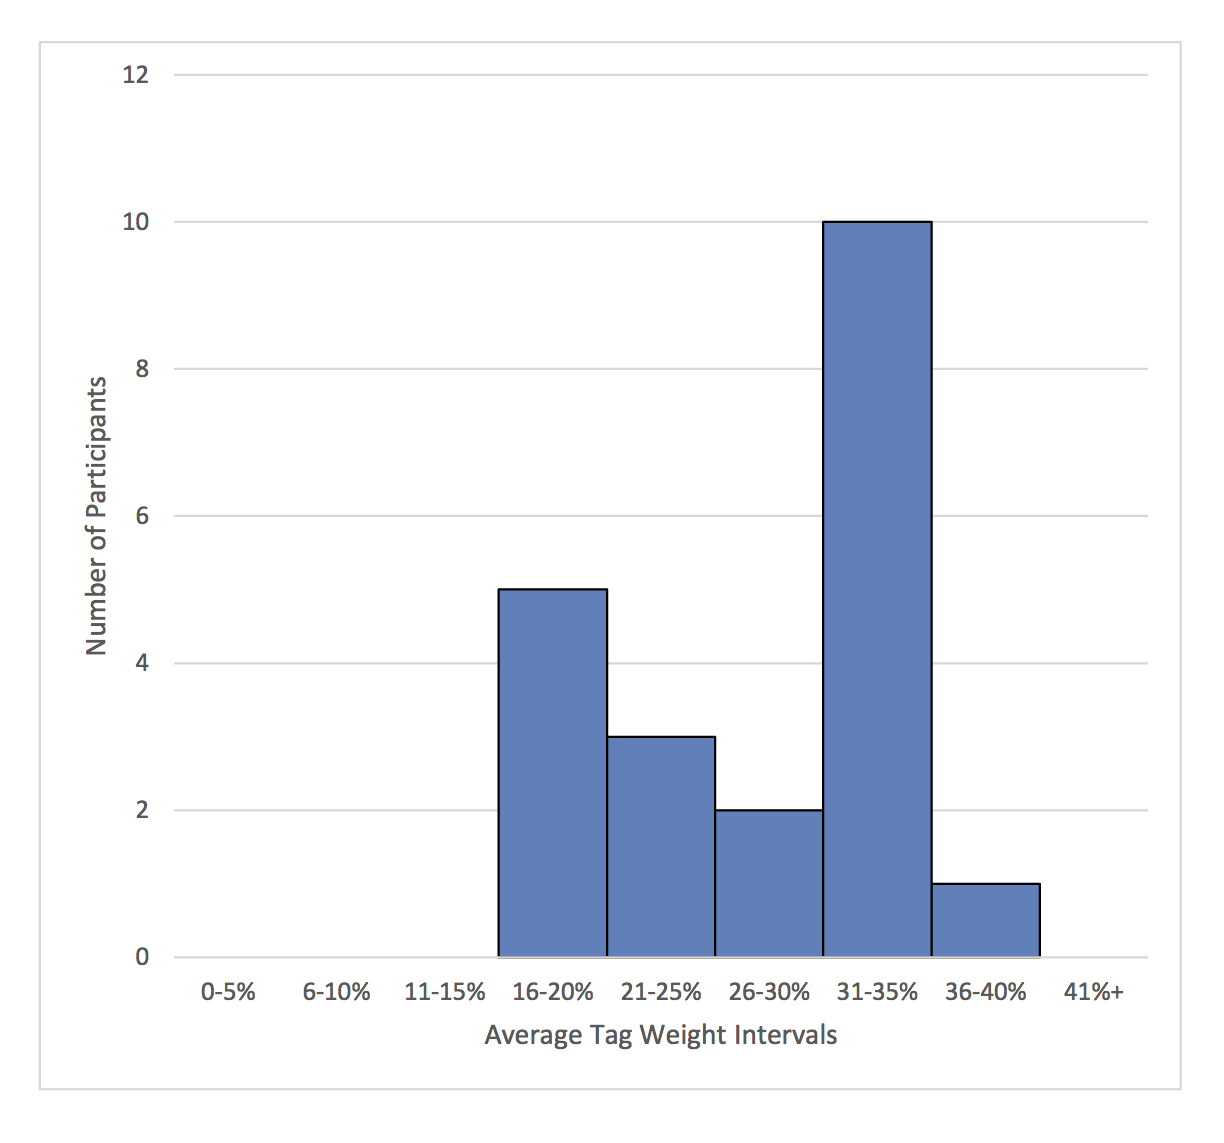
\includegraphics[scale=0.6]{pics/tag_weight_histogram.png}
\caption{Average Tag Weight Distribution among Participants}\label{fig:tag_weight_histogram}
\end{centering}
\end{figure}

\begin{figure}[!h]
\begin{centering}
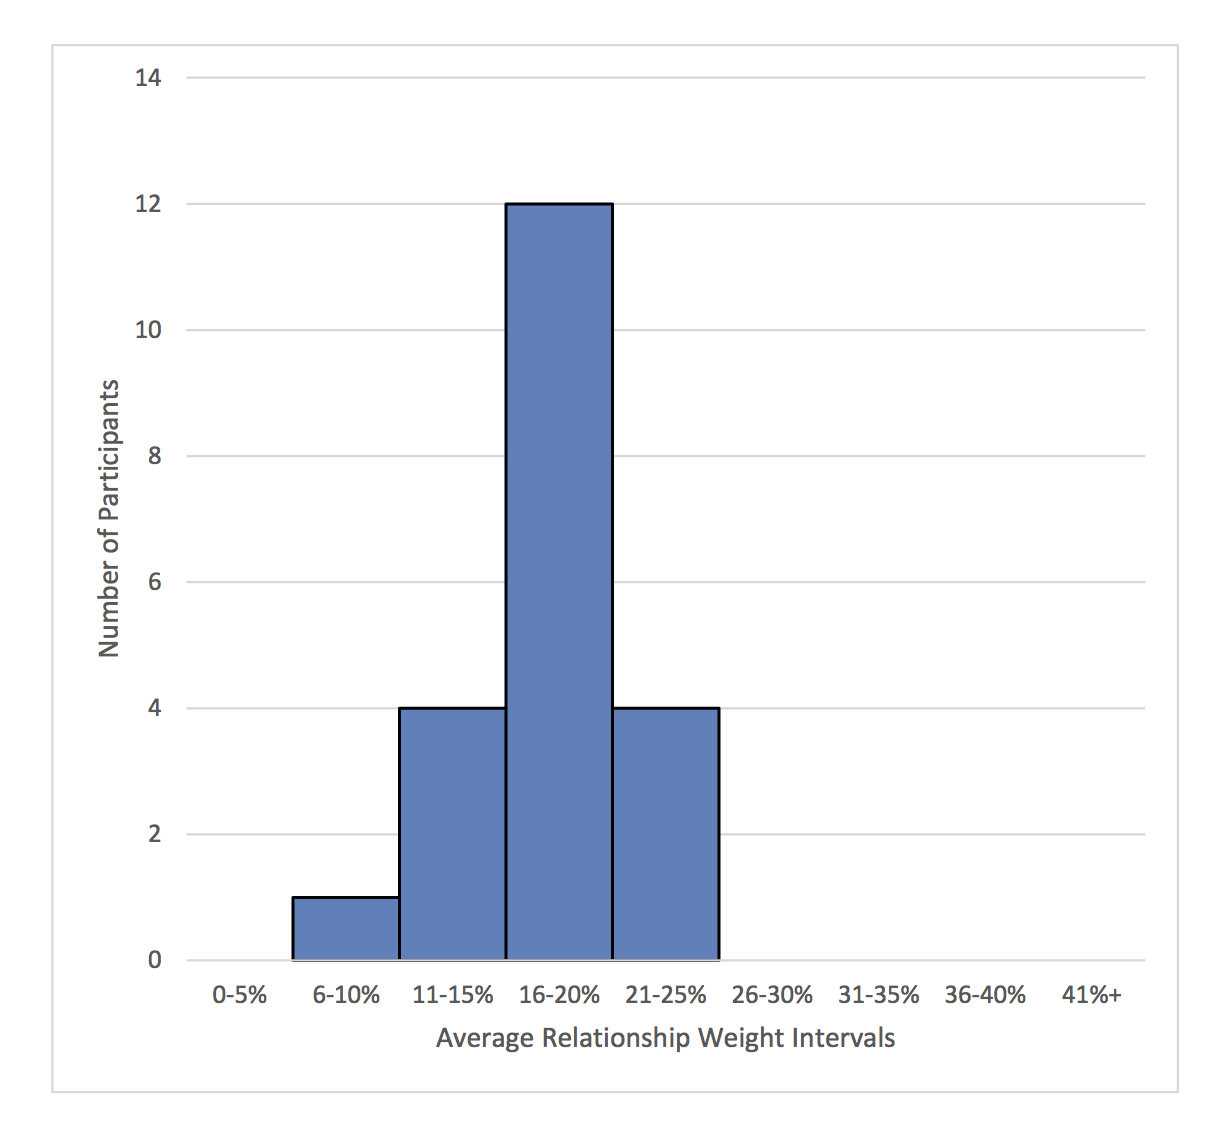
\includegraphics[scale=0.6]{pics/relationship_weight_histogram.png}
\caption{Average Relationship Weight Distribution among Participants}\label{fig:relationship_weight_histogram}
\end{centering}
\end{figure}

\begin{figure}[!h]
\begin{centering}
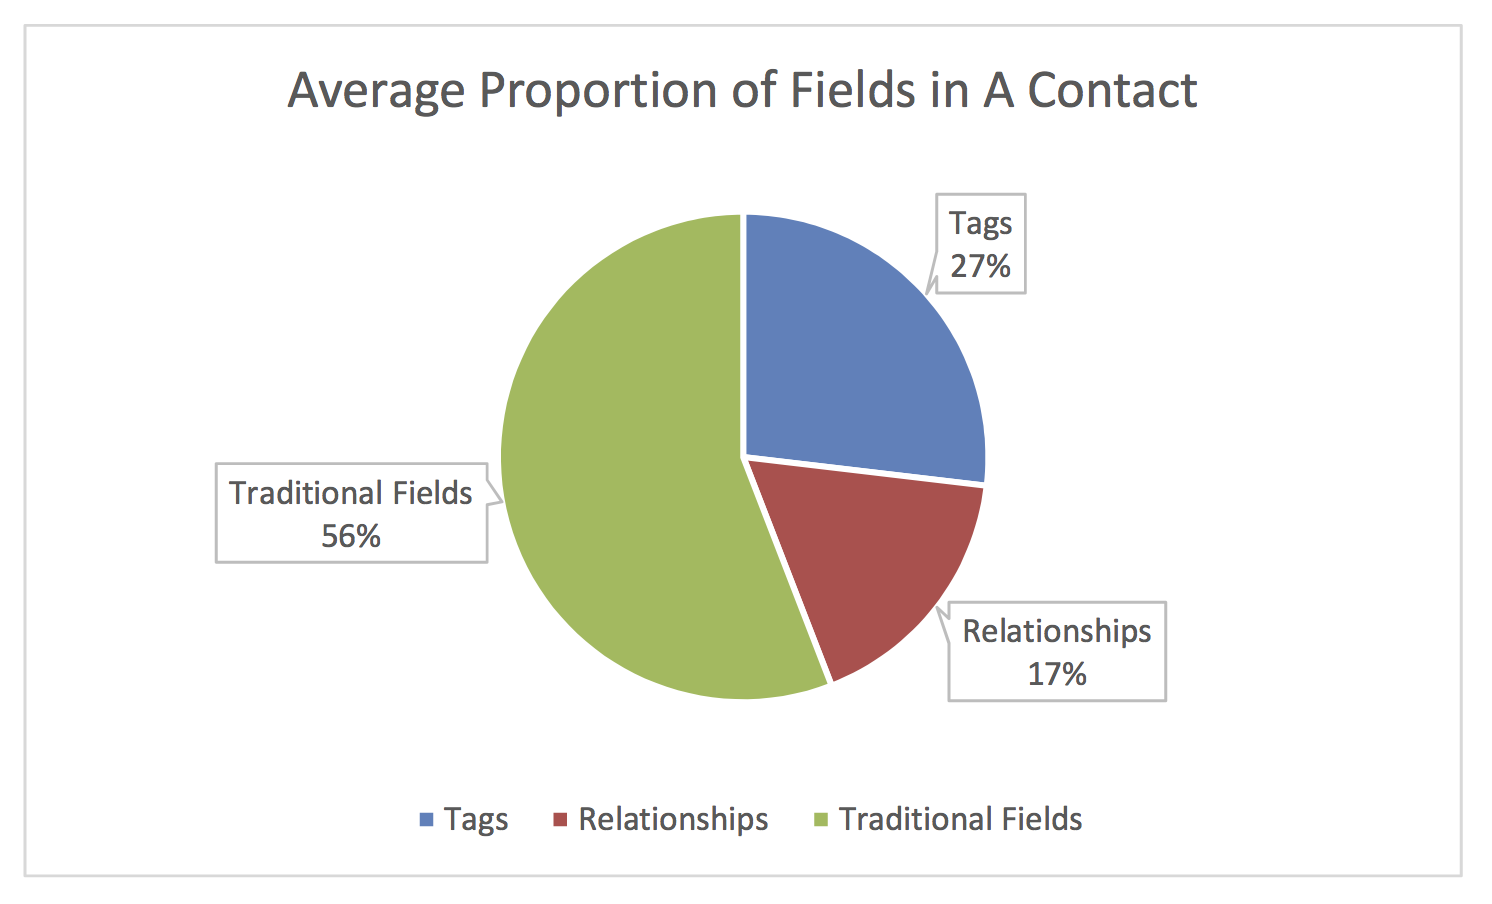
\includegraphics[scale=0.65]{pics/average_contact_fields.png}
\caption{Average Proportion of Fields in A Contact}\label{fig:average_contact_fields}
\end{centering}
\end{figure}

%\begin{tabular}{ | l | l | l | l | l | }
%\hline
%	Active Contact Total & Tag Total & Tag Average & Relationship Total & Relationship Average \\ \hline
%	46 & 180 & 3.9129999999999998 & 94 & 2.0434999999999999 \\ \hline
%	72 & 241 & 3.3472 & 146 & 2.0278 \\ \hline
%	55 & 127 & 2.3090999999999999 & 67 & 1.2181999999999999 \\ \hline
%	16 & 27 & 1.6875 & 30 & 1.875 \\ \hline
%	50 & 101 & 2.02 & 87 & 1.74 \\ \hline
%	9 & 22 & 2.4443999999999999 & 7 & 0.77780000000000005 \\ \hline
%	8 & 29 & 3.625 & 12 & 1.5 \\ \hline
%	49 & 165 & 3.3673000000000002 & 86 & 1.7551000000000001 \\ \hline
%	20 & 48 & 2.4 & 39 & 1.95 \\ \hline
%	18 & 69 & 3.8332999999999999 & 34 & 1.8889 \\ \hline
%	32 & 68 & 2.125 & 45 & 1.4063000000000001 \\ \hline
%	29 & 67 & 2.3102999999999998 & 33 & 1.1378999999999999 \\ \hline
%	23 & 60 & 2.6086999999999998 & 29 & 1.2608999999999999 \\ \hline
%	24 & 47 & 1.9582999999999999 & 38 & 1.5832999999999999 \\ \hline
%	30 & 102 & 3.4 & 58 & 1.9333 \\ \hline
%	63 & 207 & 3.2856999999999998 & 128 & 2.0316999999999998 \\ \hline
%	8 & 26 & 3.25 & 10 & 1.25 \\ \hline
%	52 & 111 & 2.1345999999999998 & 80 & 1.5385 \\ \hline
%	41 & 85 & 2.0731999999999999 & 71 & 1.7317 \\ \hline
%	22 & 41 & 1.8635999999999999 & 41 & 1.8635999999999999 \\ \hline
%	17 & 56 & 3.2940999999999998 & 31 & 1.8234999999999999 \\ \hline
%	Average & \  & \  & \  & \  \\ \hline
%	32.571399999999997 & 89.476200000000006 & 2.7262 & 55.523800000000001 & 1.6351 \\ \hline
%\end{tabular}

\subsection{Search Pattern}\label{results_search}
\subsection{General Feedbacks and Discussion}\label{results_feedbacks}
\subsection{Summary}\label{results_summary}

%\section{Database Synchronization Performance (Will Remove)}
%To evaluate the performance of our synchronization technique, we plan to use Apache Bench and Xamarin to do several load tests on the server such as excuting 1000 requests, processing up to 10 requests concurrently. The results will be measured in milliseconds and compared with other services like Gmail Contacts. 

%We will also benchmark the speed and capacity of the mobile SQLite database. In our Graphy system, the SQLite database runs on the mobile devices and communicates with Xamarin - a cross-platforms development environment. Therefore, the performance of the database can be lower than using a native development environment.

%However, due to the limitation of time and resources, we have not been able to cover all metrics listed above and the user data collected was small. On the collected data, there are some promising results in Custom Tags Weight and Relationship Weight which are shown in Table \ref{tb:experiment}. Although the experiment is still small thus not really comprehensive, it represents a common pattern in users' behaviors: The majority of contacts only contain 2 to 3 fields including the person's name, his/her phone numbers, and his/her organization. Therefore, when the users create custom tags or relationships, the weight of these pieces of information are certainly high. Regarding the performance of Graphy, the database design and the synchronization technique perform very well on the basic daily usage.
%
%\begin{table}[!ht]
%\centering
%\caption{Experiment Results}\label{tb:experiment}
%\begin{tabular}{| l | l | l | l |} \hline
%Criteria & Person 1 & Person 2 & Person 3\\ \hline
%Average CTW & 27.13\% & 22.67\% & 24.84\%\\ \hline
%Average RW & 13.61\% & 19.33\% & 18.32\%\\ \hline
%\end{tabular}
%\end{table}
